% Source code initially created by Philip Empl, sourced from Jan Küster that is open sourced under the MIT License (MIT) 2019.
% Repository: <https://github.com/philipempl/modern-latex-cv>

\documentclass[10pt,A4,english]{article}	


%----------------------------------------------------------------------------------------
%	ENCODING
%----------------------------------------------------------------------------------------

% we use utf8 since we want to build from any machine
\usepackage[utf8]{inputenc}		
\usepackage[USenglish]{isodate}
\usepackage{fancyhdr}
\usepackage[numbers]{natbib}

%----------------------------------------------------------------------------------------
%	LOGIC
%----------------------------------------------------------------------------------------

% provides \isempty test
\usepackage{xstring, xifthen}
\usepackage{enumitem}
\usepackage[italian]{babel}
\usepackage{blindtext}
\usepackage{pdfpages}
\usepackage{changepage}

%----------------------------------------------------------------------------------------
%	FONT BASICS
%----------------------------------------------------------------------------------------

% some tex-live fonts - choose your own

%\usepackage[defaultsans]{droidsans}
%\usepackage[default]{comfortaa}
%\usepackage{cmbright}
\usepackage[default]{raleway}
%\usepackage{fetamont}
%\usepackage[default]{gillius}
%\usepackage[light,math]{iwona}
%\usepackage[thin]{roboto} 

% set font default
\renewcommand*\familydefault{\sfdefault} 	
\usepackage[T1]{fontenc}

% more font size definitions
\usepackage{moresize}

%----------------------------------------------------------------------------------------
%	FONT AWESOME ICONS
%---------------------------------------------------------------------------------------- 

% include the fontawesome icon set
\usepackage{fontawesome}

% use to vertically center content
% credits to: http://tex.stackexchange.com/questions/7219/how-to-vertically-center-two-images-next-to-each-other
\newcommand{\vcenteredinclude}[1]{
    \begingroup
        \setbox0=\hbox{\includegraphics{#1}}%
        \parbox{\wd0}{\box0}
    \endgroup
}

\newcommand{\tab}[1]{
    \hspace{.2\textwidth}\rlap{#1}
}

% use to vertically center content
% credits to: http://tex.stackexchange.com/questions/7219/how-to-vertically-center-two-images-next-to-each-other
\newcommand*{\vcenteredhbox}[1]{
    \begingroup
        \setbox0=\hbox{#1}\parbox{\wd0}{\box0}
    \endgroup
}

% icon shortcut
\newcommand{\icon}[3] { 							
	\makebox(#2, #2){\textcolor{maincol}{\csname fa#1\endcsname}}
}	


% icon with text shortcut
\newcommand{\icontext}[4]{ 						
	\vcenteredhbox{\icon{#1}{#2}{#3}}  \hspace{2pt}  \parbox{0.9\mpwidth}{\textcolor{#4}{#3}}
}

% icon with website url
\newcommand{\iconhref}[5]{ 						
    \href{#4}{\vcenteredhbox{\icon{#1}{#2}{#5}}  \hspace{2pt} \textcolor{#5}{#3}}
}

% icon with email link
\newcommand{\iconemail}[5]{ 						
    \href{mailto:#4}{\vcenteredhbox{\icon{#1}{#2}{#5}} \hspace{2pt} {\textcolor{#5}{#3}}}
}

%----------------------------------------------------------------------------------------
%	PAGE LAYOUT  DEFINITIONS
%----------------------------------------------------------------------------------------

% page outer frames (debug-only)
% \usepackage{showframe}		

% we use paracol to display breakable two columns
\usepackage{paracol}
\usepackage{tikzpagenodes}
\usetikzlibrary{calc}
\usepackage{lmodern}
\usepackage{multicol}
\usepackage{lipsum}
\usepackage{atbegshi}
% define page styles using geometry
\usepackage[a4paper]{geometry}

% remove all possible margins
\geometry{top=1cm, bottom=1cm, left=1cm, right=1cm}

\usepackage{fancyhdr}
\pagestyle{empty}

% space between header and content
% \setlength{\headheight}{0pt}

% indentation is zero
\setlength{\parindent}{0mm}

%----------------------------------------------------------------------------------------
%	TABLE /ARRAY DEFINITIONS
%---------------------------------------------------------------------------------------- 

% extended aligning of tabular cells
\usepackage{array}

% custom column right-align with fixed width
% use like p{size} but via x{size}
\newcolumntype{x}[1]{%
>{\raggedleft\hspace{0pt}}p{#1}}%


%----------------------------------------------------------------------------------------
%	GRAPHICS DEFINITIONS
%---------------------------------------------------------------------------------------- 

%for header image
\usepackage{graphicx}

% use this for floating figures
% \usepackage{wrapfig}
% \usepackage{float}
% \floatstyle{boxed} 
% \restylefloat{figure}

%for drawing graphics		
\usepackage{tikz}			
\usepackage{ragged2e}	
\usetikzlibrary{shapes, backgrounds,mindmap, trees}

%----------------------------------------------------------------------------------------
%	Color DEFINITIONS
%---------------------------------------------------------------------------------------- 
\usepackage{transparent}
\usepackage{color}

% primary color
\definecolor{maincol}{RGB}{ 64,64,64}

% accent color, secondary
% \definecolor{accentcol}{RGB}{ 250, 150, 10 }

% dark color
\definecolor{darkcol}{RGB}{ 70, 70, 70 }
% light color
\definecolor{lightcol}{RGB}{245,245,245}
\definecolor{accentcol}{RGB}{59,77,97}
\definecolor{darkblue}{RGB}{111, 143, 175}
\definecolor{lightblue}{RGB}{31, 81, 255}


% Package for links, must be the last package used
%\usepackage{hyperref}

\usepackage[
	citecolor = lightblue,
	anchorcolor = lightblue,
	colorlinks=true,
	linkcolor=lightblue,
	linkbordercolor=lightblue,
	urlcolor=lightblue,
	urlbordercolor = lightblue,
	]{hyperref}

% \makeatletter
% \Hy@AtBeginDocument{
% 	%\def\@pdfborder{0 0 1}
% 	\def\@pdfborderstyle{/S/U/W 1}
% }
% \makeatother

% returns minipage width minus two times \fboxsep
% to keep padding included in width calculations
% can also be used for other boxes / environments
\newcommand{\mpwidth}{\linewidth-\fboxsep-\fboxsep}
	


%============================================================================%
%
%	CV COMMANDS
%
%============================================================================%

%----------------------------------------------------------------------------------------
%	 CV LIST
%----------------------------------------------------------------------------------------

% renders a standard latex list but abstracts away the environment definition (begin/end)
\newcommand{\cvlist}[1] {
	\begin{itemize}{#1}\end{itemize}
}

%----------------------------------------------------------------------------------------
%	 CV TEXT
%----------------------------------------------------------------------------------------

% base class to wrap any text based stuff here. Renders like a paragraph.
% Allows complex commands to be passed, too.
% param 1: *any
\newcommand{\cvtext}[1] {
	\begin{tabular*}{1\mpwidth}{p{0.98\mpwidth}}
		\parbox{1\mpwidth}{#1}
	\end{tabular*}
}
\newcommand{\cvtextsmall}[1] {
	\begin{tabular*}{0.8\mpwidth}{p{0.8\mpwidth}}
		\parbox{0.8\mpwidth}{#1}
	\end{tabular*}
}
%----------------------------------------------------------------------------------------
%	CV SECTION
%----------------------------------------------------------------------------------------

% Renders a a CV section headline with a nice underline in main color.
% param 1: section title
\newlength{\barw}
\newcommand{\cvsection}[1] {
	\vspace{14pt}
	\settowidth{\barw}{\textbf{\LARGE #1}}
	\cvtext{
		\textbf{\LARGE{\textcolor{darkcol}{#1}}}\\[-4pt]
		\textcolor{accentcol}{ \rule{\barw}{1.5pt} } \\
	}
}

\newcommand{\cvsubsection}[1] {
	\vspace{14pt}
	\settowidth{\barw}{\textbf{\Large #1}}
	\cvtext{
		\textbf{\Large{\textcolor{darkcol}{#1}}}\\[-4pt]
		\textcolor{accentcol}{ \rule{\barw}{1.5pt} } \\
	}
}

\newcommand{\cvheadline}[1] {
	\vspace{16pt}
	\cvtext{
		\textbf{\Huge{\textcolor{accentcol}{#1}}}\\[-4pt]
		 
	}
}

\newcommand{\cvsubheadline}[1] {
	\vspace{16pt}
	\cvtext{
		\textbf{\huge{\textcolor{darkcol}{#1}}}\\[-4pt]
		 
	}
}
%----------------------------------------------------------------------------------------
%	META SKILL
%----------------------------------------------------------------------------------------

% Renders a progress-bar to indicate a certain skill in percent.
% param 1: name of the skill / tech / etc.
% param 2: level (for example in years)
% param 3: percent, values range from 0 to 1
\newcommand{\cvskill}[3] {
	\begin{tabular*}{1\mpwidth}{p{0.72\mpwidth}  r}
 		\textcolor{black}{\textbf{#1}} & \textcolor{maincol}{#2}\\
	\end{tabular*}%
	
	\hspace{4pt}
	\begin{tikzpicture}[scale=1,rounded corners=2pt,very thin]
		\fill [lightcol] (0,0) rectangle (1\mpwidth, 0.15);
		\fill [accentcol] (0,0) rectangle (#3\mpwidth, 0.15);
  	\end{tikzpicture}%
}


%----------------------------------------------------------------------------------------
%	 CV EVENT
%----------------------------------------------------------------------------------------

% Renders a table and a paragraph (cvtext) wrapped in a parbox (to ensure minimum content
% is glued together when a pagebreak appears).
% Additional Information can be passed in text or list form (or other environments).
% the work you did
% param 1: time-frame i.e. Sep 14 - Jan 15 etc.
% param 2:	 event name (job position etc.)
% param 3: Customer, Employer, Industry
% param 4: Short description
% param 5: work done (optional)
% param 6: technologies include (optional)
% param 7: achievements (optional)
\newcommand{\cvevent}[7] {
	
	% we wrap this part in a parbox, so title and description are not separated on a pagebreak
	% if you need more control on page breaks, remove the parbox
	\parbox{\mpwidth}{
		\begin{tabular*}{1\mpwidth}{p{0.65\mpwidth}  r}
	 		\textcolor{black}{\textbf{#2}} & \colorbox{accentcol}{\makebox[0.35\mpwidth]{\textcolor{white}{\textbf{#1}}}} \\
			\textcolor{maincol}{#3} & \\
		\end{tabular*}\\[8pt]
	
		\ifthenelse{\isempty{#4}}{}{
			\cvtext{#4}\\
		}
	}
	\vspace{14pt}
}


%----------------------------------------------------------------------------------------
%	 CV META EVENT
%----------------------------------------------------------------------------------------

% Renders a CV event on the sidebar
% param 1: title
% param 2: subtitle (optional)
% param 3: customer, employer, etc,. (optional)
% param 4: info text (optional)
\newcommand{\cvmetaevent}[4] {
	\textcolor{maincol} { \cvtext{\textbf{\begin{flushleft}#1\end{flushleft}}}}

	\ifthenelse{\isempty{#2}}{}{
	\textcolor{black} {\cvtext{\textbf{#2}} }
	}

	\ifthenelse{\isempty{#3}}{}{
		\cvtext{{ \textcolor{maincol} {#3} }}\\
	}

	\cvtext{#4}\\[14pt]
}

%---------------------------------------------------------------------------------------
%	QR CODE
%----------------------------------------------------------------------------------------

% Renders a qrcode image (centered, relative to the parentwidth)
% param 1: percent width, from 0 to 1
\newcommand{\cvqrcode}[1] {
	\begin{center}
		\includegraphics[width={#1}\mpwidth]{qrcode}
	\end{center}
}


% HEADER AND FOOOTER 
%====================================
\newcommand\Header[1]{%
\begin{tikzpicture}[remember picture,overlay]
\fill[accentcol]
  (current page.north west) -- (current page.north east) --
  ([yshift=50pt]current page.north east|-current page text area.north east) --
  ([yshift=50pt,xshift=-3cm]current page.north|-current page text area.north) --
  ([yshift=10pt,xshift=-5cm]current page.north|-current page text area.north) --
  ([yshift=10pt]current page.north west|-current page text area.north west) -- cycle;
\node[font=\sffamily\bfseries\color{white},anchor=west,
  xshift=0.7cm,yshift=-0.32cm] at (current page.north west)
  {\fontsize{12}{12}\selectfont {#1}};
\end{tikzpicture}%
}

\newcommand\Footer[1]{%
\begin{tikzpicture}[remember picture,overlay]
\fill[lightcol]
  (current page.south east) -- (current page.south west) --
  ([yshift=-80pt]current page.south east|-current page text area.south east) --
  ([yshift=-80pt,xshift=-6cm]current page.south|-current page text area.south) --
  ([xshift=-2.5cm,yshift=-10pt]current page.south|-current page text area.south) --	
  ([yshift=-10pt]current page.south east|-current page text area.south east) -- cycle;
\node[yshift=0.32cm,xshift=9cm] at (current page.south) {\fontsize{10}{10}\selectfont \textbf{\thepage}};
\end{tikzpicture}%
}


%=====================================
%============================================================================%
%
%
%
%	DOCUMENT CONTENT
%
%
%
%============================================================================%
\begin{document}

\columnratio{0.31}
\setlength{\columnsep}{2.2em}
\setlength{\columnseprule}{4pt}
\colseprulecolor{white}


% LEBENSLAUF HIERE
\AtBeginShipoutFirst{\Header{CV IT}\Footer{1}}
\AtBeginShipout{\AtBeginShipoutAddToBox{\Header{CV IT}\Footer{2}}}

\newpage

\colseprulecolor{lightcol}
\columnratio{0.31}
\setlength{\columnsep}{2.2em}
\setlength{\columnseprule}{4pt}
\begin{paracol}{2}


\begin{leftcolumn}
%---------------------------------------------------------------------------------------
%	META IMAGE
%----------------------------------------------------------------------------------------

% personal picture
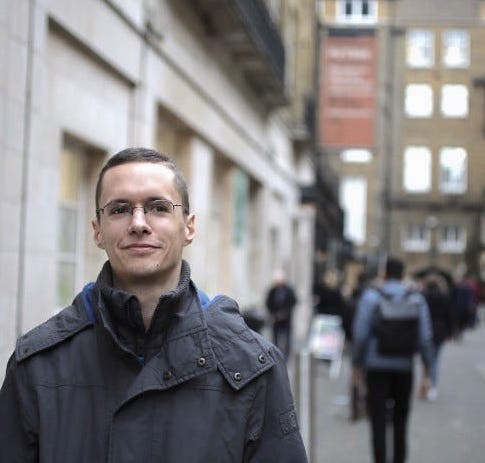
\includegraphics[width=\linewidth]{../images/sebastiano.jpg}
% QR code if no picture is allowed
%
\includegraphics[width=\linewidth]{../images/qr-code-linkedin.png}

%---------------------------------------------------------------------------------------
%	META SKILLS
%----------------------------------------------------------------------------------------
\fcolorbox{white}{white}{\begin{minipage}[c][1.5cm][c]{1\mpwidth}
	\LARGE{\textbf{\textcolor{maincol}{Sebastiano Ferraris}}} \\[2pt]
	\normalsize{ 
        \textcolor{maincol} {Geospatial Data Scientist, PhD} 
    }
\end{minipage}} \\

% \icontext{CaretRight}{12}{London, since 2014}{black}\\[6pt]
% \icontext{CaretRight}{12}{Italian nationality}{black}\\[6pt]
%\icontext{CaretRight}{12}{unmarried}{black}\\[6pt]

\cvsection{Contatti}

\icontext{MapMarker}{16}{Londra}{black}\\[6pt]
% \icontext{MobilePhone}{16}{+44 775689xxxx}{black}\\[6pt]
\iconemail{Envelope}{16}{sebastiano.ferraris@gmail.com}{sebastiano.ferraris@gmail.com}{black}\\[5pt]
\iconhref{Home}{16}{github.io/GeoDsBlog/}{https://sebastianof.github.io/GeoDsBlog/}{black}\\[5pt]
\iconhref{Github}{16}{github.com/SebastianoF}{https://www.github.com/SebastianoF}{black}\\[5pt]
\iconhref{Linkedin}{16}{linkedin.com/in/ibis-redibis/}{https://www.linkedin.com/in/ibis-redibis/}{black}\\[5pt]
\iconhref{Google}{16}{Google Scholar}{https://scholar.google.com/citations?user=1tAeAI0AAAAJ&hl=en}{black}\\[5pt]
\iconhref{GraduationCap}{16}{Research Gate}{https://www.researchgate.net/profile/Sebastiano_Ferraris}{black}\\[5pt]


\cvsection{Skillset}

\cvskill{Software development} {9+ years} {1} \\[-2pt]

\cvskill{Data science} {9+ years} {1} \\[-2pt]

\cvskill{Algorithms} {9+ years} {1} \\[-2pt]

\cvskill{Artificial intelligence} {4+ years} {0.63} \\[-2pt]

\cvskill{Geospatial Data Science} {3+ years} {0.5} \\[-2pt]

\cvskill{Medical image analysis} {4 years} {0.45} \\[-2pt]

\cvskill{Discrete Events Simulation} {1 year} {0.4} \\[-2pt]

\cvskill{Dynamic pricing} {1 year} {0.33} \\[-2pt]



\newpage
%---------------------------------------------------------------------------------------
%	EDUCATION
%----------------------------------------------------------------------------------------
\cvsection{Titoli Accademici}

\cvmetaevent
{2015 - 2018}
{PhD, Centre for Doctoral Training (EPSRC), Medical Imaging}
{University College London}
{\textit{MRI • Pre-clinical studies • Numerical methods for Image registration • 8 Papers published • 12 repositories open sourced}}

\cvmetaevent
{2014 - 2015}
{Master of Research (MRes), Medical Imaging}
{University College London}
{\textit{Numerical methods for image registration • Digital Image Processing • Optics in Medicine}}

\cvmetaevent
{2010 - 2013}
{Master of Science (MSci), Mathematics}
{Universita degli studi di Torino}
{\textit{Geometry • Error correcting code theory • Computational modelling}.}

\cvmetaevent
{2006 - 2010}
{Bachelor's of Science (BSc), Mathematics}
{Universita degli studi di Torino}
{}

%
%\cvsection{Projekte}

%	\cvlist{
%		\item \hyperlink{https://github.com/philipempl/ether-twin}{\textbf{Ether-Twin.}}\\ Ethereum Applikation für Digital Twins.
%		\item \hyperlink{https://github.com/philipempl/Peter-Pan}{\textbf{Peter Pan.}}\\ Koch-App (t.b.a.).
%		\item \hyperlink{https://github.com/philipempl/Innovation-Tool}{\textbf{Innovation Tool.}}\\ Webcrawler für \hyperlink{https://ibi.de/}{Ibi}.
%		\item \hyperlink{https://github.com/philipempl/cozone}{\textbf{COZONE.}} \\ Soziales Netzwerk (t.b.a.).
%		\item \hyperlink{https://github.com/geritwagner/enlit}{\textbf{ENLIT.}}\\ Exploring new Literature (Bachelorarbeit).
%		\item \textbf{Crowdfunding.} \\Modul mit \hyperlink{https://senacor.com/}{Senacor} für \hyperlink{https://www.paydirekt.de/}{paydirekt}.
%		}

\cvsection{Volontariato}

\icontext{GraduationCap}{12}{Maths Tutor, \href{https://actiontutoring.org.uk/}{Action Tutoring}}{black}\\[6pt]
\icontext{ClockO}{12}{Scanner and Marshall, \href{https://www.parkrun.org.uk/}{Parkrun}}{black}\\[6pt]




	
%\cvqrcode{0.3}

\end{leftcolumn}
\begin{rightcolumn}
%---------------------------------------------------------------------------------------
%	TITLE  HEADER
%----------------------------------------------------------------------------------------


%---------------------------------------------------------------------------------------
%	PROFILE
%----------------------------------------------------------------------------------------
\cvsection{Breve introduzione}
\vspace{4pt}

Ricercatore e scienziato dei dati, con pubblicazioni su riviste scientifiche internazionali, ho lavorato e fatto ricerca in molteplici settori, come industria dell'auto, analisi di immagini mediche, bancario, prezzatura dinamica e scienza dei dati geotemporali.\\

In questi stettori ho risolto problemi tecnici usando algoritmi, modellistica matematica, simulazione, data processing, analisi dei colli di bottiglia, studio delle prestazioni e dell'affidabilità. Sono specializzato nella creazione rapida di prototipi completi, testati e production ready, nella loro presentazione ad un pubblico diversificato, stakeholders o neofiti, e nella consegna ai team di sviluppatori, per la loro distribuzione su vasta scala.


%---------------------------------------------------------------------------------------
%	WORK EXPERIENCE
%----------------------------------------------------------------------------------------

\vspace{10pt}
\cvsection{Esperienze}
\vspace{4pt}


\cvevent
{June 2020 - today}
	{Data scientist | \href{https://www.generalsystem.com/}{General System}}
	{Geospatial data Science Services: Startup in stealth mode until April 2022}
	{
		• Sviluppo di prototipi per automatizzare l'analisi dei dati spaziotemporali con metodi di clustering, creazione di dashboard e visualizzazioni con \href{https://kepler.gl/}{KeplerGl}  visualisation.\\
		• Collaborazione con clienti e esperti per integrare nuove features e richieste nei prototipi durante lo sviluppo. \\
		• Consegna dei prototipi ai team di sviluppo (Devs) e distribuzione (DevSecOps). \\
		• Sviluppato e reso \href{https://github.com/thegeneralsystem}{open source} librerie in python per dare agli utenti strumenti ed esempi per utilizzare il prodotto creato: \href{https://www.generalsystem.com/product}{Data Flow Index}.\\
		• Contribuito al \href{https://www.generalsystem.com/blog}{blog aziendale} dedicato alla creazione di una comunità di utenti ed appassionati attorno al tema della scienza dei dati geospaziale. \\
	}
\vfill\null


\cvevent
{Sept 2019 - June 2020}
	{Algorithm Engineer | \href{https://www.paceup.com/}{Pace}}
	{Dynamic pricing for the hospitality industry}
	{
		• Nel team di simulaizone validazione, dedicato a testare le pipeline ETL e gli algoritmi portanti.\\
		• Mantenimento del codice in produzione ed integrazione di nuove features.\\
	}
\vfill\null

	
\cvevent
{Oct 2018 - June 2019}
	{Back End Developer | \href{https://www.thoughtmachine.net/}{Thought Machine} }
	{Cloud native core banking}
	{
		• Lavorato con lo stato dell'arte delle infrastrutture in cloud per distribuire microservizi in un ambiente cloud-agnostico: Python, Go, Docker, Kubernetes, e customizzazioni derivate.\\
		• Mantenimento e miglioramento delle CI/CD e dei processi di release.\\
	}
\vfill\null

\cvevent
{Sept 2014 - Sept 2018}
	{MRes + PhD in Medical Image analysis | \href{https://www.ucl.ac.uk/medical-physics-biomedical-engineering/study/postgraduate-research/medical-imaging-mres-mphilphd}{UCL} }
	{Research Student}
	{
		• Pre-clinical trial sugli effetti dell'amministrazione di steroidi per le nascite premature come parte di un team multi-disciplinare ed internazionel.\\
		• Pubblicato \href{https://scholar.google.com/citations?user=1tAeAI0AAAAJ&hl=en}{7 articoli peer-reviewed} anche su \href{https://www.sciencedirect.com/science/article/pii/S1053811918305366?via\%3Dihub}{Neuroimage} 
		e su \href{https://www.nature.com/articles/s41598-019-39922-8}{Nature Scientific Report} su \href{https://www.cv-foundation.org/openaccess/content_cvpr_2016_workshops/w15/papers/Ferraris_Accurate_Small_Deformation_CVPR_2016_paper.pdf}{diffeomorphic image registration} e \href{https://www.sciencedirect.com/science/article/pii/S1053811918305366?via\%3Dihub}{Machine Learning per l'automatizzaione delle segmentazioni di immagini a risonanza magnetica}.\\
		• Sostenitore di criteri di rproducibilità nella ricerca: creato e reso open sourced 12 librerie in Python (\href{https://discovery.ucl.ac.uk/id/eprint/10072833/}{Sec 7.2.2 of della mia tesi di dottorato}), e reso pubblico un \href{https://zenodo.org/record/1289776}{dataset di micro-MRI}.\\
	}
\vfill\null


\cvevent
{March 2013 - June 2014}
	{Industrial Simulation Modeller | \href{https://www.simtec-group.eu/it/}{SimTec} }
	{Automotive industry, discrete events simulation}
	{
		• Modelli di simulazione di flusso per body in white, verniciature ed assemblaggi per stimare l'efficienza, rimuovere colli di bottiglia, dimensionare buffers, dare supporto alla creazione dei layout degli impianti per diversi clienti sia in Italia che in Germania.\\
		• Creato un algoritmo di cammino minimo per la logistica interna ed esterna per le parti di assemblaggio, dalle baie di carico alla linea.\\
		• Presentato al primo meeting annuale di Tecnomatix Plant Simulation User Conference a Stoccarda. \\
	}
\vfill\null


\cvevent
{June 2011 - Oct 2011}
	{Developer | \href{https://www.tc-web.it}{TcWeb}  }
	{Web development and technology consulting}
	{
		• Contratto a termine come sviluppatore junior in Java, Java J2EE, Struts 2, Uml. \\
		• Sviluppatore di algoritmi: creato e sviluppato il prototipo di un algoritmo ungherese generalizzato per il parsing delle pagine di giornale. \\
	}
\vfill\null


% \cvevent
% {Sept 2006 - June 2014}
% 	{Bachelor + Master in Mathematics | \href{https://en.unito.it/}{UNITO}   }
% 	{Web development and technology consulting}
% 	{
% 		• Graduated in Mathematics with specialisation in Computational Geometry..\\
% 		•  Master of Science in Mathematics with a \href{https://www.matematicamente.it/tesi/Ferraris-Winograd.pdf}{Thesis} about the applications of the Winograd transform to error correcting codes.\\
% 	}
% \vfill\null



\cvsection{Pubblicazioni selezionate}

\begin{itemize}[leftmargin=*]
\item Ferraris S, van der Merwe J, Van Der Veeken L, Prados F, Iglesias JE, Melbourne A, Lorenzi M, Modat M, Gsell W, Deprest J, Vercauteren T. 
\href{https://www.ncbi.nlm.nih.gov/pmc/articles/PMC6203700/}{"A magnetic resonance multi-atlas for the neonatal rabbit brain"}.
Neuroimage. \textit{Neuroimage} 2018 Oct doi: 10.1016/j.neuroimage.2018.06.029.
\item van der Merwe J, van der Veeken L, Ferraris S, Gsell W, Himmelreich U, Toelen J, Ourselin S, Melbourne A, Vercauteren T, Deprest J.  
\href{https://www.nature.com/articles/s41598-019-39922-8}{"Early neuropathological and neurobehavioral consequences of preterm birth in a rabbit model"}. 
In: \textit{Nature scientific reports}, May 2019.
\item Ferraris S, Lorenzi M, Daga P, Modat M, Vercauteren T. 
\href{https://ieeexplore.ieee.org/document/7789554}{"Accurate small deformation exponential approximant to integrate large velocity fields: Application to image registration"}. 
In: \textit{Proceedings of the IEEE Conference on Computer Vision and Pattern Recognition}, Lipsum, June 12-17, 2020.
\item Ferraris S, Shakir ID, Van Der Merwe J, Gsell W, Deprest J, Vercauteren T 
\href{https://joss.theoj.org/papers/10.21105/joss.00354}{"Bruker2nifti: Magnetic resonance images converter from bruker ParaVision to NIfTI format"}. 
In: \textit{Journal of Open Source Software}, 2017.
\item Ferraris S 
\href{https://discovery.ucl.ac.uk/id/eprint/10072833/}{"Image computing tools for the investigation of the neurological effects of preterm birth and corticosteroid administration"} 
\textit{PhD thesis, University College London}, 2019.


\end{itemize}
% hofixes to create fake-space to ensure the whole height is used
\mbox{}
\vfill
Potete trovare la mia lista completa di pubblicazioni sul mio profilo di \href{https://scholar.google.com/citations?user=1tAeAI0AAAAJ&hl=en}{Google Scholar}.
\mbox{}
\vfill
\mbox{}
\vfill
\mbox{}
\vfill
\mbox{}
\vfill
\mbox{}
\vfill
\mbox{}
\vfill
\mbox{}
\vfill
\mbox{}
\vfill
\mbox{}
\vfill
\mbox{}
\vfill
\mbox{}
\vfill
\mbox{}
\vfill
\mbox{}
\vfill
\mbox{}
\vfill
\mbox{}


\today     \hspace{1cm}   \hrulefill

\hspace*{30mm}\phantom{Lorem, \today }~~~~~~~~~~~~~~~~~~~~~~~~~~~Sebastiano Ferraris

\end{rightcolumn}
\end{paracol}


\end{document}
